\chapter{Objektno orijentirano programiranje}

\section{Enkapsulacija}


Sadržaj \textit{Student.h} datoteke:

\begin{minted}{C++}
#pragma once
#include <map>
#include <string>

struct Student {
	std::string ime, prezime, jmbag;
	std::map<std::string,unsigned> ocjene;
	
	Student(std::string,std::string,std::string);
	bool ocijeni(std::string, unsigned);
	bool upis_kolegija(std::string);
	void info();
};
\end{minted}


Sadržaj \textit{Student.cpp} datoteke:

\begin{minted}{C++}
#include <cctype>
#include <cstdlib>
#include <iostream>
#include <map>
#include <string>
#include <utility>

#include "Student.h"

using namespace std;

Student::Student(string i, string p, string j)
	: ime(i), prezime(p) {
		if(j.length() != 10)
			exit(-1);
		for(int k = 0; k < 10; ++k)
			if(!isdigit(j[k]))
				exit(-2);
		jmbag = j;
}

bool Student::ocijeni(string k, unsigned o) {
	if(ocjene.find(k) == ocjene.end())
		return false; // nema upisan taj kolegij
	if(o > 5)
		exit(-3);
	ocjene[k] = o;
	return true;
}

bool Student::upis_kolegija(std::string k) {
	if(ocjene.find(k) != ocjene.end())
		return false; // vec ima upisan taj kolegij
	ocjene[k]; // ne treba ocjene[k] = 0;
	return true;
}

void Student::info() {
	cout << "Ime:     " << ime     << endl
		 << "Prezime: " << prezime << endl
		 << "JMBAG:   " << jmbag   << endl
		 << "Ocjene:"   << endl;
	if(ocjene.empty() == true)
		cout << "\t nema upisanih kolegija"
				  << endl;
	else {
		map<string,unsigned>::iterator it;
		for(it = ocjene.begin(); it != ocjene.end(); ++it) {
			cout << "\tkolegij: " << it->first 
					  << ",\t";
			if(it->second == 0)
				cout << "nema ocjene";
			else
				cout << "ocjena: " << it->second;
			cout << endl;
		}
	}
	cout << endl;
}
\end{minted}


Sadržaj \textit{Zaposlenik.h} datoteke:

\begin{minted}{C++}
#include <set>
#include <string>

class Zaposlenik {
private:
std::string ime, prezime;
    double placa;
    std::set<std::string> kolegiji;
public:
    Zaposlenik(std::string,std::string,double);
    bool dodaj_kolegij(std::string);
};
\end{minted}


Sadržaj \textit{Zaposlenik.cpp} datoteke:

\begin{minted}{C++}
#include <set>
#include <string>

using namespace std;

Zaposlenik::Zaposlenik(string i, string p, double pl)
    : ime(i), prezime(p), placa(pl) { }

bool Zaposlenik::dodaj_kolegij(string k) {
    return kolegiji.insert(k).second;
}
\end{minted}


Sadržaj \textit{main.cpp} datoteke:

\begin{minted}{C++}
#include <iostream>
#include "Student.h"

using namespace std;

int main(void) {
    Student j("John", "Doe", "0123456789");
    j.info();
    j.upis_kolegija("Linearna");
    j.upis_kolegija("Analiza");
    j.ocijeni("Analiza", 5);
    j.ocijeni("Linearna", 4);
    j.info();

    return 0;
}
\end{minted}


Enkapsulacija predstavlja proces objedinjavanja podataka (atributa) 
i funkcija (metoda) koje rade nad tim podacima unutar jedne cjeline koju nazivamo klasom. 
Jedan od važnih ciljeva je kontrola nad time kojim dijelovima klase korisnik može izravno pristupiti.
Takvim kontroliranim pristupom podacima povećava se sigurnost programskog koda
jer korisnik može koristiti samo javno dostupno sučelje
klase (metode kroz koje se osigurava da podaci ne poprime neispravne vrijednosti).
Korisnik klase ne mora znati na koji su način podaci pohranjeni ili kako su pojedine operacije implementirane.
\medskip

Kontrola pristupa članovima klase ostvaruje se pomoću \textbf{modifikatora pristupa}.
U ovoj točki promotrit ćemo sljedeća dva modifikatora pristupa:
\texttt{private} i \texttt{public}.
Članovi deklarirani kao \textbf{\texttt{private}} dostupni su samo unutar same klase.
Članovi deklarirani kao \textbf{\texttt{public}} dostupni su iz bilo kojeg dijela programa koji ima pristup objektu.
\medskip

Primjerice, promotrimo strukturu \texttt{Datum}
koja sprema podatke o danu, mjesecu i godini.
\begin{minted}{C++}
struct Datum {
    int dan, mjesec, godina;
};
\end{minted}
No, sad korisnik može izvršavanjem sljedećeg koda spremiti
kao vrijednosti atributa datuma sljedeće vrijednosti
(koje ne predstavljaju ispravan datum):
\begin{minted}{C++}
    Datum datum;
    datum.dan = datum.mjesec = datum.godina = 123;
\end{minted}
Stoga dodajemo klasi metodu \texttt{provjeri} koja će provjeriti ispravnost datuma
te metodu \texttt{postavi} kojom se omogućuje postavljanje datuma
samo ako vrijednosti dana, mjeseca i godine predstavljaju ispravan datum.
Te metode vraćaju podatak o tome je li datum ispravan,
odnosno jesmo li uspješno promijenili datum.
\begin{minted}{C++}
struct Datum {
private:
    int dan, mjesec, godina;
    bool provjeri(int d, int m, int g);
public:
    bool postavi(int d, int m, int g);
};
\end{minted}
Budući da su dan, mjesec i godina deklarirani unutar sekcije private, njima nije moguće pristupiti izravno izvan strukture.
Pomoćna funkcija \texttt{provjeri} je također privatna budući da je riječ o pomoćnoj funkciji
za koju korisnik ne mora znati da postoji. 
Korisniku je na raspolaganju javna funkcija \texttt{postavi},
koja predstavlja dio sučelja strukture
(tj.\ ono što korisnik može koristiti). 
\medskip

U objektno orijentiranom programiranju češće se koristi \texttt{class},
pa ćemo i mi tako ubuduće češće pisati \texttt{class}
umjesto \texttt{struct}.
Sljedeće je isto kao u prethodnom primjeru:
\begin{minted}{C++}
class Datum {
private:
    int dan, mjesec, godina;
    bool provjeri(int d, int m, int g);
public:
    bool postavi(int d, int m, int g);
};
\end{minted}
Ključna razlika između \texttt{struct} i \texttt{class} je u zadanoj razini pristupa članovima: 
kod \texttt{struct} je ona po \textit{defaultu} \texttt{public}, dok je kod \texttt{class} ona \texttt{private}.
Obzirom da objekti obično skrivaju svoje podatke i izlažu samo javno sučelje, prirodnije je kao zadani pristup (pomoću \texttt{class}) staviti kao \texttt{private}. Time se smanjuje mogućnost da se slučajno zaboravi napisati \texttt{private}.
Ključna riječ \texttt{struct} koristi se za jednostavne podatkovne tipove
čiji svi članovi mogu biti javni.


\begin{zadatak}\label{zad:klase-student-zaposlenik}
    Promijenite strukture \texttt{Student} i \texttt{Zaposlenik}
    iz \textcolor{red}{zadataka ... i ...}
    u klase.
    Odredite modifikatore pristupa za atribute i metode tih klasa.
\end{zadatak}


\begin{rjesenje}
Za klasu \texttt{Student}:
\begin{minted}[
        linenos,
        numbersep=5pt
    ]{C++}
class Student {
private:
    std::string ime, prezime, jmbag;
    std::map<std::string,unsigned> ocjene;
public:
    Student(std::string,std::string,std::string);
    bool ocijeni(std::string, unsigned);
    bool upis_kolegija(std::string);
    void info();
};
\end{minted}

Za klasu \texttt{Zaposlenik}:
\begin{minted}[
        linenos,
        numbersep=5pt
    ]{C++}
class Zaposlenik {
private:
    std::string ime, prezime;
    double placa;
    std::set<std::string> kolegiji;
public:
    Zaposlenik(std::string,std::string,double);
    bool dodaj_kolegij(std::string);
};
\end{minted}
\end{rjesenje}

\begin{razmisljanje}
    \begin{enumerate}
        \item 
        Zašto ne trebamo mijenjati implementaciju metode \texttt{upis\_kolegija},
        tj.\ zašto možemo u implementaciji te metode
        koristiti preslikavanje \texttt{ocjene}
        koje je u klasi \texttt{Student}
        označeno kao \texttt{private}?

        Podsjetnik na metodu \texttt{upis\_kolegija} klase \texttt{Student}:
    \begin{minted}[
        linenos,
        numbersep=5pt
    ]{C++}
bool Student::upis_kolegija(std::string k) {
    if(ocjene.find(k) != ocjene.end())
        return false;
    ocjene [k];
    return true; 
}
    \end{minted}

    \item 
    Objasnite koje su posljedice pri upotrebi klase \texttt{Student} za evidenciju
    studenata na fakultetu ako izmijenimo klasu \texttt{Student}
    iz rješenja prethodnog zadatka na sljedeći način:
\begin{minted}[
        linenos,
        numbersep=5pt
    ]{C++}
struct Student {
private:
    std::string ime, prezime, jmbag;
    std::map<std::string,unsigned> ocjene;
public:
    Student(std::string,std::string,std::string);
    bool ocijeni(std::string, unsigned);
private:
    bool upis_kolegija(std::string);
public: // ne želimo da i info bude private
    void info();
};
\end{minted}
    Također, što bi se dogodilo kada bismo konstruktor klase \texttt{Student}
    označili kao privatan?

    \item 
    Smatrate li da je za jednostavan par koji ima x i y koordinatu
bolje pisati:
\begin{minted}[
        linenos,
        numbersep=5pt
    ]{C++}
struct par {
    double x, y;
};
\end{minted}
ili ovako:
\begin{minted}[
        linenos,
        numbersep=5pt
    ]{C++}
class par {
public:
    double x, y;
};
\end{minted}
    \end{enumerate}
\end{razmisljanje}


U programskom jeziku C++ funkcije mogu imati 
\textbf{defaultne argumente} (poznate i pod nazivom 
\textbf{pretpostavljeni parametri}). 
To su vrijednosti koje će se automatski koristiti ako prilikom poziva funkcije korisnik ne navede odgovarajući argument.
Primjerice, sljedeća funkcija ima defaultni argument:
\begin{minted}{C++}
void ispisiPoruku(std::string poruka = "Dobar dan!") {
    cout << poruka;
}
\end{minted}

Funkciju možemo pozvati na dva načina:
\begin{minted}{C++}
ispisiPoruku("Kako ste?");
ispisiPoruku();
\end{minted}

U prvom pozivu funkcija će ispisati tekst \texttt{"Kako ste?"}, dok će u drugom pozivu ispisati tekst 
\texttt{"Dobar dan!"}.
Isti princip može se primijeniti i na konstruktore klasa.


\begin{zadatak}\label{zad:racuni}
    Implementirati klasu \texttt{Racun} koja predstavlja bankovni račun s iznosom izraženim u eurima te mogućnošću prikaza njegove protuvrijednosti u švicarskim francima (CHF).
    Klasa treba sadržavati sljedeće podatke o računu:
    ime vlasnika računa, iznos na računu izražen u eurima te iznos tečaja za pretvorbu iz EUR u CHF.
    
    Implementirajte metodu
    \texttt{double pretvori()}
    za pretvorbu iznosa iz eura u švicarske franke.
    Zatim implementirajte metodu
    \texttt{void info()} koja pomoću metode \texttt{pretvori} na standardni izlaz ispisuje ime vlasnika računa, iznos u eurima te
    odgovarajući iznos u švicarskim francima nakon pretvorbe.
    Korisnik klase ne treba znati da metoda \texttt{pretvori} postoji.
    
    Omogućite stvaranje objekata tipa \texttt{Racun} uz zadavanje imena vlasnika, iznosa i tečaja, pri čemu ime vlasnika treba imati zadanu vrijednost 
    \texttt{"nepoznat"}, a tečaj zadanu vrijednost 1.
    Koristite inicijalizacijsku listu konstruktora.

    Sučelje spremite u datoteku \textit{Racun.h},
    a implementaciju u datoteku \textit{Racun.cpp}.
    Napišite u \textit{main.cpp} datoteci
    primjer programa za testiranje.
\end{zadatak}


\begin{rjesenje}
Kako korisnik ne bi izravno mogao pristupati i nekontrolirano mijenjati
podatke koje pamtimo o računu,
deklariramo \texttt{ime}, \texttt{iznos} i \texttt{tecaj}
kao privatne dijelove klase.
Metoda \texttt{pretvori} također je privatna jer predstavlja pomoćnu funkciju koja služi za internu obradu podataka. Korisnik klase ne mora znati kako se pretvorba obavlja, već samo koristiti 
metodu \texttt{info} za ispis podataka o računu na ekran.
Konstruktor mora biti javan kako bi se objekti klase mogli stvarati izvan klase.
\medskip

Prema tome, sadržaj \texttt{Racun.h} datoteke je sljedeći:

\begin{minted}[
        linenos,
        numbersep=5pt
    ]{C++}
#pragma once
#include <string>

class Racun {
private:
    std::string ime;
    double iznos, tecaj;
    double pretvori();
public:
    Racun(double iz, std::string im = "nepoznat",
          double t = 1);
    void info();
};
\end{minted}

U gornjem kodu smo pri deklaraciji konstruktora koristili pretpostavljene vrijednosti parametara 
\texttt{im} i \texttt{t}.
Te vrijednosti navodimo samo u deklaraciji funkcije
(u ovom slučaju, konstruktora) - u implementaciji
(u datoteci \textit{Racun.cpp}) ih ne navodimo ponovo.
Sada je sadržaj \textit{Racun.cpp} datoteke,
uz upotrebu inicijalizacijske liste konstruktora, sljedeći:

\begin{minted}[
        linenos,
        numbersep=5pt
    ]{C++}
#include <iostream>
#include <string>
#include "Racun.h"

using namespace std;

double Racun::pretvori() {
	return iznos * tecaj;
}

Racun::Racun(double iz, string im, double t) 
    : ime(im), iznos(iz), tecaj(t) {}

void Racun::info() {
    cout << ime << endl 
         << '\t' << iznos << "EUR" << endl
         << '\t' << pretvori() << "CHF" << endl;
}
\end{minted}


Jedan mogući sadržaj \textit{main.cpp} datoteke s programom za testiranje:

\begin{minted}[
        linenos,
        numbersep=5pt
    ]{C++}
#include <iostream>
#include "Racun.h"

using namespace std;

int main(void) {
    Racun r1(100.99,"John",0.95),
          r2(123.23,"Mary"), // tecaj jednak 1 
          r3(0.12); // ime jednako "nepoznat" i tecaj jednak 1
    r1.info();
    r2.info();
    r3.info();
    return 0;
}
\end{minted}

U gornjem kodu, kod objekta \texttt{r2} treći argument nije naveden, zbog čega se koristi pretpostavljena vrijednost 1.
Slično kod objekta \texttt{r3} drugi argument nije naveden,
zbog čeka se koristi pretpostavljena vrijednost \texttt{"nepoznat"}.
\end{rjesenje}


\begin{razmisljanje}
    \begin{enumerate}
        \item 
    Zašto nismo parametre pri deklaraciji konstruktora naveli u sljedećem poretku:
    \begin{minted}[
        linenos,
        numbersep=5pt
    ]{C++}
Racun(std::string im = "nepoznat", double iz, 
      double t = 1);
    \end{minted}
    Objasnite grešku koja je nastala na sljedećem primjeru te izvedite zaključak
    o poretku parametara u deklaraciji funkcije:
    \begin{minted}[
        linenos,
        numbersep=5pt
    ]{C++}
Racun r2(123.23);
    \end{minted}

    \item 
    Objasnite zašto sada ne možemo klasi \texttt{Racun} dodati i sljedeći konstruktor
    (možete upotrijebiti primjer s objektom \texttt{r2} iz prethodnog pitanja):
    \begin{minted}[
        linenos,
        numbersep=5pt
    ]{C++}
Racun(double iz) : iznos(iz) {}
    \end{minted}
    \end{enumerate}
\end{razmisljanje}



\section{Upotreba \texttt{this} pokazivača}

Sadržaj \texttt{racun.h} datoteke:

\begin{minted}{C++}
#pragma once
#include <string>

class Racun {
private:
	static int broj_racuna;
	std::string ime;
	double iznos; // u EUR
	static double tecaj; // za pretvorbu u CHF
	double pretvori() const; // iznos iz EUR u CHF
public:
	Racun(double iz, std::string im = "nepoznat");
	Racun(const Racun& r);
	void info() const;
	static int koliko();
	static void promijeni(double t);
	~Racun();
};
\end{minted}


Sadržaj \texttt{Racun.cpp} datoteke:

\begin{minted}{C++}
#include <iostream>
#include <string>
#include "Racun.h"

using namespace std;

double Racun::tecaj = 0.94;
int Racun::broj_racuna = 0;

Racun::Racun(double iz, string im)
	: ime(im), iznos(iz) {
		++broj_racuna;
	}

double Racun::pretvori() const {
	return iznos * tecaj;
}


void Racun::promijeni(double t) {
	//NE: cout << iznos << endl;
	if(t >= 0.9 && t <= 1)
		tecaj = t;
}

void Racun::info() const {
	cout << this->ime << endl
		 << '\t' << this->iznos << "EUR" << endl
		 << '\t' << this->pretvori() << "CHF" << endl;
}

Racun::~Racun() {
	--broj_racuna;
}

int Racun::koliko() {
	return broj_racuna;
}

Racun::Racun(const Racun& r)
 	: ime(r.ime), iznos(r.iznos) {
	++broj_racuna;
}

\end{minted}



Sadržaj \texttt{main.cpp} datoteke:

\begin{minted}{C++}
#include <iostream>
#include "Racun.h"

using namespace std;

void funkcija(const Racun* r) {
	r->info();
	cout << r->koliko() << endl;
}

int main(void) {
	cout << Racun::koliko() << endl;
	//cout << Racun::tecaj << endl;
	Racun::promijeni(0.91);
	const Racun primjer(100,"test");
	funkcija(&primjer);
	{
	Racun r1(100.99,"John"),
	r2(123.23,"Mary");
	r1.info();
	//r1.tecaj = 100;
	r1.promijeni(0.99);
	r2.info();
	cout << Racun::koliko() << endl;
	funkcija(&r1);
	funkcija(&r2);
	}
	cout << Racun::koliko() << endl;
	return 0;
}
\end{minted}



\section{Nasljeđivanje}


\textbf{Nasljeđivanje} predstavlja mehanizam kojim se među klasama uspostavlja hijerarhijski odnos. 
Primjerice, promotrimo klase 
\texttt{Knjiga} i \texttt{Mobitel}
koje neka internetska trgovina koristi kako bi radila s podacima o 
knjigama i mobitelima koje prodaje.
Obje klase imaju niz zajedničkih atributa i metoda, 
poput atributa naziv, cijena, popust, količina na skladištu
te metode za prikaz cijene s obračunatim popustom.
Kako bi izbjegli dupliciranje koda, preciznije,
ponavljanje definiranja podataka u svakoj klasi posebno,
bolji je pristup definirati zajedničku klasu \texttt{Proizvod}
koja sadrži sve zajedničke atribute klase \texttt{Knjiga}
i klase \texttt{Mobitel}
te metode koje su od koristi za obje te klase.
Kao što je prikazano na slici \ref{fig:hijerarhija_proizvoda}, time dobivamo
hijerarhiju u kojoj klase
\texttt{Knjiga} i \texttt{Mobitel} nasljeđuju zajedničke članove klase
\texttt{Proizvod}.
\medskip

\begin{figure}[htbp]
\centering
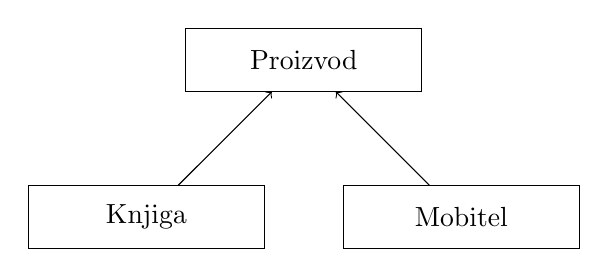
\begin{tikzpicture}[
    class/.style={
        draw,
        rectangle,
        minimum width=3cm,
        minimum height=0.8cm
    }
]

\node[class] (proizvod) {Proizvod};
\node[class] (knjiga) at (-2,-2) {Knjiga};
\node[class] (mobitel) at (2,-2) {Mobitel};

\draw[->] (knjiga) -- (proizvod);
\draw[->] (mobitel) -- (proizvod);

\end{tikzpicture}
\caption{Hijerarhija klasa koja prikazuje nasljeđivanje u sustavu internetske trgovine.}
\label{fig:hijerarhija_proizvoda}
\end{figure}

Klasa \texttt{Proizvod} naziva se \textbf{bazna klasa}, dok se klase 
\texttt{Student} i \texttt{Zaposlenik} nazivaju 
\textbf{izvedene klase}. 
Bazna klasa definira članove koji su zajednički svim objektima u hijerarhiji, dok izvedene klase dodaju samo svoje specifične članova
(poput broja stranica za knjigu ili kapaciteta memorije za mobitel).
\medskip

Pri pisanju koda, izvedene klase moraju navesti koju klasu (ili više klasa)
naslijeđuju u \textbf{izvedenoj listi klase}.
Tamo navodimo bazne klase uz (opcionalno) navođenje modifikatora pristupa.
Primjerice, za klasu \texttt{Knjiga}
to bismo napravili ovako:
\begin{minted}{C++}
class Knjiga : public Proizvod {
    ...
}
\end{minted}

Atributi bazne klase se često ne označavaju modifikatorom
pristupa \texttt{private},
nego modifikatorom pristupa \texttt{\textbf{protected}}.
Time se omogućuje da im izvedene klase mogu izravno pristupati, dok su i dalje skriveni od ostatka programa.
Također, treba istaknuti da se prilikom stvaranja objekta izvedene klase 
prvo se mora inicijalizirati bazni dio objekta. 
Zato izvedeni konstruktor poziva konstruktor bazne klase pomoću inicijalizacijske liste.
Primjerice, pretpostavimo da konstruktor klase \texttt{Knjiga}
prima naziv, što je dio bazne klase koja ima konstruktor koji prima naziv proizvoda, te broj stranica.
Tada bismo implementaciju konstruktora klase \texttt{Knjiga} izveli ovako:
\begin{minted}{C++}
Knjiga::Knjiga(std::string naziv, unsigned br_str)
    : Proizvod(naziv), broj_stranica(br_str) {
        ...
}
\end{minted}



\begin{zadatak}\label{zad:hijerarhija-osoba}
    Napisati baznu klasu \texttt{Osoba} te razdvojiti njezino sučelje od implementacije u datoteke \texttt{Osoba.h} i \texttt{Osoba.cpp}. Zatim preraditi klase \texttt{Student} i \texttt{Zaposlenik} iz zadatka \ref{zad:klase-student-zaposlenik} tako da nasljeđuju klasu \texttt{Osoba}. Zajedničke atribute i metode izdvojiti u baznu klasu, dok u izvedenim klasama ostaviti samo članove specifične za studente odnosno zaposlenike.
\end{zadatak}


\begin{rjesenje}
    Zajednički atributi klasama \texttt{Student} i \texttt{Zaposlenik}
    su atributi \texttt{ime} i \texttt{prezime}.
    Prema tome ćemo dodati klasi \texttt{Osoba} te atribute,
    uz konstruktor koji će im postavljati vrijednosti.
    Atributi će imati modifikator pristupa \texttt{protected}
    kako bi ih izvedene klase mogle koristiti
    dok bi oni za korisnika bili i dalje nedostupni.
    Sadržaj datoteke \texttt{Osoba.h} je sljedeći:

    \begin{minted}[
        linenos,
        numbersep=5pt
    ]{C++}
#pragma once

#include <string>

class Osoba {
protected:
    std::string ime, prezime;
public:
    Osoba(std::string im, std::string prez);
};
    \end{minted}

    Sadržaj datoteke \texttt{Osoba.cpp}
    (sadrži implementaciju konstruktora klase \texttt{Osoba}:

\begin{minted}[
        linenos,
        numbersep=5pt
    ]{C++}
#include <string>
#include "Osoba.h"

using namespace std;

Osoba::Osoba(string im, string prez) 
    : ime(im), prezime(prez) { }
\end{minted}

Za klase \texttt{Student} i klase \texttt{Zaposlenik} 
postavimo da nasljeđuju klasu \texttt{Osoba}
te im uklonimo
atribute \texttt{ime} i \texttt{prezime}
(obzirom da ih sad nasljeđuju iz bazne klase \texttt{Osoba}).
Također treba u datotekama vezanim uz sučelje i implementacije
izvedenih klasa \texttt{Student} i \texttt{Zaposlenik} uključiti \textit{Osoba.h} datoteku. 
Izmijenjeni sadržaj datoteke \textit{Student.h}:
\begin{minted}[
        linenos,
        numbersep=5pt
    ]{C++}
...
#include "Osoba.h"

class Student : public Osoba {
private:
    std::string jmbag; // uklonili smo ime i prezime
    ...
};
\end{minted}

Izmijenjeni sadržaj datoteke \textit{Zaposlenik.h}:
\begin{minted}[
        linenos,
        numbersep=5pt
    ]{C++}
...
#include "Osoba.h"

class Zaposlenik : public Osoba {
private:
    // uklonili smo ime i prezime
    double placa;
    ...
};
\end{minted}

Izmijenimo konstruktor izvedene klase \texttt{Student}
(u \textit{Student.cpp} datoteci, u kojoj također
uključimo \textit{Osoba.h} datoteku)
tako da poziva konstruktor bazne klase \texttt{Osoba}:
\begin{minted}[
        linenos,
        numbersep=5pt
    ]{C++}
...
#include "Osoba.h"
...
Student::Student(string im, string prez, string jmb)
  : Osoba(im, prez) {
    ...
}
\end{minted}

Slično izmijenimo konstruktor izvedene klase \texttt{Zaposlenik}
(u \textit{Zaposlenik.cpp} datoteci, u kojoj također
uključimo \textit{Osoba.h} datoteku):
\begin{minted}[
        linenos,
        numbersep=5pt
    ]{C++}
...
#include "Osoba.h"
...
Zaposlenik::Zaposlenik(string im, string prez, double pl)
    : Osoba(im, prez), placa(pl) { }
\end{minted}

Uočite da ostatak kod ne treba mijenjati, primjerice,
u metodi \texttt{info} izvedene klase \texttt{Student}
i dalje možemo koristiti atribut 
\texttt{ime} koje je ta klasa naslijedila iz bazne klase \texttt{Osoba}:
\begin{minted}[
        linenos,
        numbersep=5pt
    ]{C++}
void Student::info() {
    cout << "Ime: " << ime << endl
    ...
}
\end{minted}
\end{rjesenje}


\begin{razmisljanje}
    \begin{enumerate}
        \item 
        Obrazložite zašto se kod uz ovakvu implementaciju
        konstruktora izvedene klase \texttt{Zaposlenik} iz prethodnog zadatka ne može uspješno kompajlirati:
        \begin{minted}{C++}
Zaposlenik::Zaposlenik(string im, string prez, double pl)
    : placa(pl) {
        ime = im;
        prezime = prez;
}
        \end{minted}
    \end{enumerate}
\end{razmisljanje}


Što se tiče konverzija, objekt izvedene klase može se automatski pretvoriti u objekt, referencu ili pokazivač na baznu klasu. 
Obrnuta konverzija nije dopuštena bez eksplicitne konverzije.
Primjerice, promotrimo hijerarhiju klasa sa slike \ref{fig:hijerarhija_proizvoda}.
Ako je objekt \texttt{knjiga} tipa klase \texttt{Knjiga}
tada je samo prva od sljedeće dvije linije koda ispravna:
\begin{minted}{C++}
Proizvod proizvod = knjiga; // ispravno
Knjiga druga_knjiga = proizvod; // nije ispravno
\end{minted}
Takve konverzije vrlo su korisne kada želimo pisati općenite funkcije koje rade s različitim vrstama proizvoda. 
Primjerice, možemo definirati funkciju koja prima objekt, referencu ili pokazivač na \texttt{Proizvod}, 
a onda toj funkciji prosljeđivati i knjige i mobitele bez potrebe za pisanjem zasebnih verzija funkcije za svaki tip proizvoda.

\begin{zadatak}\label{zad:osoba-zaposlenik-student}
    U zadatku \ref{zad:hijerarhija-osoba} napisana je klasa \texttt{Osoba}
    te klase \texttt{Zaposlenik} i \texttt{Student}
    koje nasljeđuju tu klasu, a pamte podatke o pojedinim
    zaposlenicima i studentima fakulteta.
    Fakultet organizira izlet te ima popis osoba koje su na izlet prijavljene
    (neke od tih osoba su studenti, a neke zaposlenici).
    Napišite (globalnu) funkciju 
    \begin{center}
        \texttt{void popis\_sudionika(Osoba* popis, int duljina)}
    \end{center}
    koja prima niz osoba duljine \texttt{duljina}
    te za svaku ispisuje njeno ime i prezime
    (po potrebi dodajte metode odgovarajućim klasama).
    Napišite i program za testiranje.
\end{zadatak}


\begin{rjesenje}
    Obzirom da su atributi \texttt{ime} i \texttt{prezime}
    označeni kao privatni, dodajemo u sučelje klase \texttt{Osoba} metodu za ispis imena i prezimena.
    Dodamo njenu deklaraciju u klasu \texttt{Osoba}
    (u \textit{Osoba.h} datoteci):
    \begin{minted}[
        linenos,
        numbersep=5pt
    ]{C++}
class Osoba {
    ...
public:
    void osnovne_info();
    ...
};
    \end{minted}
    Implementaciju te metode dodamo u \textit{Osoba.cpp}
    datoteku:
\begin{minted}[
        linenos,
        numbersep=5pt
    ]{C++}
void Osoba::osnovne_info() {
    cout << "Ime: " << ime << endl
         << "Prezime: " << prezime << endl;
}
\end{minted}

    Sadržaj \textit{main.cpp} datoteke s implementacijom
    tražene funkcije i primjer programa za testiranje
    (u \texttt{main} funkciji):
\begin{minted}[
        linenos,
        numbersep=5pt
    ]{C++}
#include <iostream>
#include "Osoba.h"
#include "Student.h"
#include "Zaposlenik.h"

using namespace std;

void popis_sudionika(Osoba* popis, int duljina) {
    cout << "Popis:" << endl;
    for(int i = 0; i < duljina; ++i)
        popis[i].osnovne_info();
}

int main(void) {
    Osoba b("Bob", "Smith");
    Student j("John", "Doe", "0123456789");
    Zaposlenik z("Jane", "Doe", 1400);
    Osoba osobe[] = { b, j, z };
    popis_sudionika(osobe, 3);
    
    return 0;
}
\end{minted}
\end{rjesenje}


\begin{zadatak}
    Dodajte konstruktorima i destruktorima klasa \texttt{Osoba},
    \texttt{Student} i \texttt{Zaposlenik} iz zadatka \ref{zad:osoba-zaposlenik-student}
    ispis odgovarajuće poruke na ekran
    o pozivu konstruktora ili destruktora za tu klasu, poput
    poruke \texttt{"Poziv konstruktora za osobu."}
    Izvedite zaključak o tome kojim se redoslijedom pozivaju konstruktori i destruktori pri upotrebi izvedenih klasa.
\end{zadatak}

\begin{rjesenje}
    Dodajemo deklaracije destruktora u klase \texttt{Osoba}, \texttt{Student} i \texttt{Zaposlenik},
    te dodajemo ispis odgovarajuće poruke u konstruktore
    i destruktore tih klasa.
    \medskip
    
    U datoteci \textit{Osoba.h} dodajmo deklaraciju destruktora klase \texttt{Osoba}:
    \begin{minted}[
        linenos,
        numbersep=5pt
    ]{C++}
class Osoba {
    ...
    ~Osoba();
};
    \end{minted}
    U datoteci \textit{Student.h} dodajmo deklaraciju destruktora klase \texttt{Student}:
    \begin{minted}[
        linenos,
        numbersep=5pt
    ]{C++}
class Student : public Osoba {
    ...
    ~Student();
};
    \end{minted}
    U datoteci \textit{Zaposlenik.h} dodajmo deklaraciju destruktora klase \texttt{Zaposlenik}:
    \begin{minted}[
        linenos,
        numbersep=5pt
    ]{C++}
class Zaposlenik : public Osoba {
    ...
    ~Zaposlenik();
};
    \end{minted}
    Dodajemo u \textit{Osoba.cpp} datoteku ispis poruke pri pozivu konstruktora klase \texttt{Osoba}
    te implementaciju destruktora te klase s ispisom odgovarajuće poruke:
    \begin{minted}[
        linenos,
        numbersep=5pt
    ]{C++}
Osoba::Osoba(string im, string prez) : ... {
    cout << "Konstruktor osobe." << endl;
}

Osoba::~Osoba() {
    cout << "Destruktor osobe." << endl;
}
    \end{minted}
    Dodajemo u \textit{Student.cpp} datoteku ispis poruke pri pozivu konstruktora klase \texttt{Student}
    te implementaciju destruktora te klase s ispisom odgovarajuće poruke:
    \begin{minted}[
        linenos,
        numbersep=5pt
    ]{C++}
Student::Student(...) : ... {
    cout << "Konstruktor studenta." << endl;
    ...
}

Student::~Student() {
    cout << "Destruktor studenta." << endl;
}
    \end{minted}
    Dodajemo u \textit{Zaposlenik.cpp} datoteku ispis poruke pri pozivu konstruktora klase \texttt{Zaposlenik}
    te implementaciju destruktora te klase s ispisom odgovarajuće poruke:
    \begin{minted}[
        linenos,
        numbersep=5pt
    ]{C++}
Zaposlenik::Zaposlenik(...) : ... {
    cout << "Konstruktor zaposlenika." << endl;
    ...
}

Zaposlenik::~Zaposlenik() {
    cout << "Destruktor zaposlenika." << endl;
}
    \end{minted}
    Ako je \texttt{main} funkcija sljedeća:
\begin{minted}[
        linenos,
        numbersep=5pt
    ]{C++}
int main(void) {
    Student j("John", "Doe", "0123456789");
    Zaposlenik z("Jane", "Doe", 1400);
    
    return 0;
}
\end{minted}
    tada dobivamo nakon kompajliranja i pokretanja programa sljedeći ispis:
    \medskip
    
    \hspace*{2em}\texttt{Konstruktor osobe.\\
    \hspace*{2em}Konstruktor studenta.\\
    \hspace*{2em}Konstruktor osobe.\\
    \hspace*{2em}Konstruktor zaposlenika.\\
    \hspace*{2em}Destruktor zaposlenika.\\
    \hspace*{2em}Destruktor osobe.\\
    \hspace*{2em}Destruktor studenta.\\
    \hspace*{2em}Destruktor osobe.}
    \medskip

    Kod stvaranja objekta izvedene klase najprije se poziva konstruktor bazne klase, a zatim konstruktor izvedene klase. Razlog tome je što se bazni dio objekta mora inicijalizirati prije nego što se može inicijalizirati dio koji pripada izvedenoj klasi.
    \medskip
    
    S druge strane, pri uništavanju objekta redoslijed je obrnut. Najprije se poziva destruktor izvedene klase, a zatim destruktor bazne klase. Time se osigurava da se najprije oslobode resursi specifični za izvedenu klasu, a tek nakon toga resursi bazne klase.
\end{rjesenje}


\section{Polimorfizam}


\textbf{Polimorfizam} omogućuje da se objekti \textbf{različitih} izvedenih klasa koriste preko zajedničkog sučelja definiranog baznom klasom. 
Time se postiže veća fleksibilnost i proširivost programa jer se ista operacija može različito ponašati ovisno o stvarnom tipu objekta nad kojim se izvršava.
\medskip

Polimorfizam se ostvaruje pomoću \textbf{virtualnih funkcija}
- funkcija članica bazne klase koje su deklarirane ključnom riječi 
\texttt{virtual}. 
Kada izvedena klasa redefinira (engl.\ \textit{override}) virtualnu funkciju istog prototipa, 
omogućuje se dinamičko povezivanje funkcijskih poziva tijekom izvođenja programa.
\medskip 

Ako se objektu pristupa preko \textbf{pokazivača} ili \textbf{reference} na baznu klasu, 
poziv virtualne funkcije neće biti određen tipom pokazivača ili reference, već stvarnim tipom objekta. 
U tom slučaju izvršit će se odgovarajuća implementacija funkcije iz izvedene klase.
\medskip

\begin{zadatak}
    U zadatku \ref{zad:osoba-zaposlenik-student} definirana je klasa \texttt{Osoba}
    te klase \texttt{Student} i \texttt{Zaposlenik}
    koje nasljeđuju tu klasu.
    Napišite globalnu funkciju (u \texttt{main.cpp} datoteci)
    \begin{center}
        \texttt{void popis\_sudionika(Osoba** popis, int duljina)}
    \end{center}
    koja prima popis osoba
    (od kojih su neki studenti, a neki zaposlenici)
    koje sudjeluju na nekoj konferenciji u obliku niza pokazivača na objekte tipa \texttt{Osoba}
    te duljinu tog niza.
    Funkcija za svaku osobu s popisa ispisuje ime i prezime, a ako je riječ o osobi koja je ujedno i student,
    tada još ispisuje i preostale podatke o studentu 
    (JMBAG te podatke o ocjenama upisanih kolegija).
    Napišite i neki program za testiranje (u \texttt{main} funkciji).
\end{zadatak}


\begin{rjesenje}
    Potrebno je dodati klasi \texttt{Osoba} i klasi \texttt{Student}
    metodu istog prototipa, primjerice, prototipa
    \begin{center}
        \texttt{void info()}
    \end{center}
    koja ispisuje tražene podatke o osobi odnosno o studentu.
    Pritom ćemu tu metodu dodati samo klasi \texttt{Osoba} gdje ona treba biti 
    označena kao virtualna
    (jer u klasi \texttt{Student} već imamo takvu metodu).
    Tada će tražena funkcija \texttt{popis\_sudionika} biti implementirana ovako:
    \begin{minted}[
        linenos,
        numbersep=5pt
    ]{C++}
void popis_sudionika(Osoba** popis, int duljina) {
    cout << "Popis:" << endl;
    for(int i = 0; i < duljina; ++i)
        popis[i] -> info();
}
    \end{minted}

    U sučelje klase \texttt{Osoba} (u datoteci \texttt{Osoba.h}) dodamo deklaraciju funkcije \texttt{info} koju označimo s ključnom riječi \texttt{virtual}:

    \begin{minted}[
        linenos,
        numbersep=5pt
    ]{C++}
class Osoba {
    ...
public:
    virtual void info();
    ...
};
    \end{minted}

    Implementaciju te funkcije dodamo u datoteku \texttt{Osoba.cpp}.
    Funkcija ispisuje podatke koje imamo spremljene za svaku osobu, tj.\ njeno ime i prezime:
\begin{minted}[
        linenos,
        numbersep=5pt
    ]{C++}
void Osoba::info() {
    cout << "Ime: "     << ime     << endl 
         << "Prezime: " << prezime << endl;
}
\end{minted}
Uočite da kod implementacije te funkcije ne navodimo ključnu riječ \texttt{virtual}!

Program za testiranje može biti sljedeći:
\begin{minted}[
        linenos,
        numbersep=5pt
    ]{C++}
int main(void) {
    Student student("John", "Doe", "0123456789");
    Zaposlenik zaposlenik("Jane", "Doe", 1400);
    Osoba osoba = student;
    Osoba* osobe[] = { &student, &zaposlenik, &osoba };
    popis_sudionika(osobe,3);

    return 0;
}
\end{minted}
\end{rjesenje}


\begin{razmisljanje}
    \begin{enumerate}
        \item 
        Kad bi funkciju \texttt{popis\_sudionika} iz prethodnog zadatka implementirali 
        tako da umjesto niza pokazivača na objekte tipa \texttt{Osoba}
        prima niz objekata tipa \texttt{Osoba},
        što bi ispisao sljedeći izmijenjeni program iz prethodnog rješenja za testiranje te (izmijenjene) funkcije:
        \begin{minted}[
        linenos,
        numbersep=5pt
    ]{C++}
    Osoba osobe[] = { student, zaposlenik, osoba };
    popis_sudionika(osobe,3);
\end{minted}
    Obrazložite svoj odgovor!

    \item 
    Ako bi izvedene klase \texttt{Student} i \texttt{Zaposlenik} iz prethodnog zadatka
    imale dijelove koje je dinamički potrebno alocirati,
    treba li destruktor bazne klase \texttt{Osoba} nužno označiti kao virtualan?
    Obrazložite na sljedećem primjeru:

    \begin{minted}{C++}
    Osoba* p = new Student("John","Doe","0123456789");
    delete p;
    \end{minted}
    \end{enumerate}
\end{razmisljanje}


Ponekad ne želimo stvarati objekte bazne klase jer se ona koristi isključivo kao zajedničko sučelje za izvedene klase. 
U takvim situacijama koristi se \textbf{apstraktna klasa}
 - klasa koja sadrži barem jednu \textbf{čistu virtualnu funkciju} 
(engl.\ \textit{pure virtual function}). 
 Čista virtualna funkcija deklarira se dodavanjem izraza \texttt{"= 0"} na kraj deklaracije funkcije
(čime cijela klasa kojoj ta funkcija pripada postaje apstraktna).
Za apstraktnu klasu nije moguće stvarati objekte, odnosno nije dopušteno deklarirati njezine instance. 
Međutim, moguće je koristiti pokazivače i reference na apstraktnu klasu, što omogućuje ostvarivanje polimorfizma.
\medskip
    
Izvedene klase moraju implementirati sve naslijeđene čiste virtualne funkcije 
kako i same ne bi postale apstraktne klase.


\begin{zadatak}
    U sustavu koji koristi klase \texttt{Osoba}, \texttt{Student} i
    \texttt{Zaposlenik} želimo osigurati da svaka osoba bude ili student
    ili zaposlenik. Drugim riječima,
    ne smije biti dopušteno stvarati objekte koji predstavljaju
    samo općenitu osobu.
    Izmijenite implementaciju navedenih klasa tako da se objekti klase
    \texttt{Osoba} ne mogu izravno stvarati, dok se objekti izvedenih
    klasa \texttt{Student} i \texttt{Zaposlenik} i dalje mogu normalno
    koristiti.
\end{zadatak}

\begin{rjesenje}
    Kako bi klasa \texttt{Osoba} postala apstraktna, dovoljno joj je barem jednu funkciju
    učiniti čistom virtualnom funkcijom.
    Mi ćemo to ovdje napraviti za funkciju \texttt{info} klase \texttt{Osoba}:

    \begin{minted}[
        linenos,
        numbersep=5pt
    ]{C++}
        class Osoba {
            ...
            virtual void info() = 0 ;
            ...
        };
    \end{minted}

    Izvedena klasa \texttt{Zaposlenik} u trenutnom kodu ne implementira naslijeđenu
    (sada čistu virtualnu) funkciju \texttt{void info()}
    pa je ta klasa postala apstraktna klasa.
    Kako bi to promijenili, dodamo deklaraciju te funkcije klasi \texttt{Zaposlenik}
    (u datoteci \texttt{Zaposlenik.h}):

    \begin{minted}[
        linenos,
        numbersep=5pt
    ]{C++}
    class Zaposlenik : public Osoba {
        ...
        void info();
    };
    \end{minted}

    a zatim i njenu implementaciju (u datoteku \texttt{Zaposlenik.cpp}):
    \begin{minted}[
        linenos,
        numbersep=5pt
    ]{C++}
    void Zaposlenik::info() {
        cout << "Ime: " << ime << endl
             << "Prezime: " << prezime << endl
             << "Placa: " << placa << endl
             << "Kolegiji:" << endl;
        if(kolegiji.empty())
            cout << "nema kolegija ciji je nositelj" << endl;
        else {
            set<string>::iterator it;
            for(it = kolegiji.begin(); it != kolegiji.end(); ++it)
                cout << '\t' << *it << endl;
        }
        cout << endl;
    }
    \end{minted}

    Obzirom da gornja funkcija koristi \texttt{cout} i \texttt{endl},
    potrebno je također u datoteku \texttt{Zaposlenik.h} uključiti 
    \texttt{iostream} datoteku zaglavlja:
    \begin{minted}[
        linenos,
        numbersep=5pt
    ]{C++}
        #include <iostream>
    \end{minted}
\end{rjesenje}


\begin{razmisljanje}
    \begin{enumerate}
        \item 
        Ako se vratimo funkciji \texttt{void popis\_sudionika(Osoba** popis, int duljina)}
        iz jednog od prethodnih zadataka, 
        što će sada ispisati sljedeći kod za testiranje:

        \begin{minted}{C++}
    Student student("John", "Doe", "0123456789");
    Zaposlenik zaposlenik("Jane", "Doe", 1400);
    Osoba* osobe[] = { &student, &zaposlenik };
    popis_sudionika(osobe,2);
        \end{minted}
    \end{enumerate}
\end{razmisljanje}